\documentclass[1p]{elsarticle_modified}
%\bibliographystyle{elsarticle-num}

%\usepackage[colorlinks]{hyperref}
%\usepackage{abbrmath_seonhwa} %\Abb, \Ascr, \Acal ,\Abf, \Afrak
\usepackage{amsfonts}
\usepackage{amssymb}
\usepackage{amsmath}
\usepackage{amsthm}
\usepackage{scalefnt}
\usepackage{amsbsy}
\usepackage{kotex}
\usepackage{caption}
\usepackage{subfig}
\usepackage{color}
\usepackage{graphicx}
\usepackage{xcolor} %% white, black, red, green, blue, cyan, magenta, yellow
\usepackage{float}
\usepackage{setspace}
\usepackage{hyperref}

\usepackage{tikz}
\usetikzlibrary{arrows}

\usepackage{multirow}
\usepackage{array} % fixed length table
\usepackage{hhline}

%%%%%%%%%%%%%%%%%%%%%
\makeatletter
\renewcommand*\env@matrix[1][\arraystretch]{%
	\edef\arraystretch{#1}%
	\hskip -\arraycolsep
	\let\@ifnextchar\new@ifnextchar
	\array{*\c@MaxMatrixCols c}}
\makeatother %https://tex.stackexchange.com/questions/14071/how-can-i-increase-the-line-spacing-in-a-matrix
%%%%%%%%%%%%%%%

\usepackage[normalem]{ulem}

\newcommand{\msout}[1]{\ifmmode\text{\sout{\ensuremath{#1}}}\else\sout{#1}\fi}
%SOURCE: \msout is \stkout macro in https://tex.stackexchange.com/questions/20609/strikeout-in-math-mode

\newcommand{\cancel}[1]{
	\ifmmode
	{\color{red}\msout{#1}}
	\else
	{\color{red}\sout{#1}}
	\fi
}

\newcommand{\add}[1]{
	{\color{blue}\uwave{#1}}
}

\newcommand{\replace}[2]{
	\ifmmode
	{\color{red}\msout{#1}}{\color{blue}\uwave{#2}}
	\else
	{\color{red}\sout{#1}}{\color{blue}\uwave{#2}}
	\fi
}

\newcommand{\Sol}{\mathcal{S}} %segment
\newcommand{\D}{D} %diagram
\newcommand{\A}{\mathcal{A}} %arc


%%%%%%%%%%%%%%%%%%%%%%%%%%%%%5 test

\def\sl{\operatorname{\textup{SL}}(2,\Cbb)}
\def\psl{\operatorname{\textup{PSL}}(2,\Cbb)}
\def\quan{\mkern 1mu \triangleright \mkern 1mu}

\theoremstyle{definition}
\newtheorem{thm}{Theorem}[section]
\newtheorem{prop}[thm]{Proposition}
\newtheorem{lem}[thm]{Lemma}
\newtheorem{ques}[thm]{Question}
\newtheorem{cor}[thm]{Corollary}
\newtheorem{defn}[thm]{Definition}
\newtheorem{exam}[thm]{Example}
\newtheorem{rmk}[thm]{Remark}
\newtheorem{alg}[thm]{Algorithm}

\newcommand{\I}{\sqrt{-1}}
\begin{document}

%\begin{frontmatter}
%
%\title{Boundary parabolic representations of knots up to 8 crossings}
%
%%% Group authors per affiliation:
%\author{Yunhi Cho} 
%\address{Department of Mathematics, University of Seoul, Seoul, Korea}
%\ead{yhcho@uos.ac.kr}
%
%
%\author{Seonhwa Kim} %\fnref{s_kim}}
%\address{Center for Geometry and Physics, Institute for Basic Science, Pohang, 37673, Korea}
%\ead{ryeona17@ibs.re.kr}
%
%\author{Hyuk Kim}
%\address{Department of Mathematical Sciences, Seoul National University, Seoul 08826, Korea}
%\ead{hyukkim@snu.ac.kr}
%
%\author{Seokbeom Yoon}
%\address{Department of Mathematical Sciences, Seoul National University, Seoul, 08826,  Korea}
%\ead{sbyoon15@snu.ac.kr}
%
%\begin{abstract}
%We find all boundary parabolic representation of knots up to 8 crossings.
%
%\end{abstract}
%\begin{keyword}
%    \MSC[2010] 57M25 
%\end{keyword}
%
%\end{frontmatter}

%\linenumbers
%\tableofcontents
%
\newcommand\colored[1]{\textcolor{white}{\rule[-0.35ex]{0.8em}{1.4ex}}\kern-0.8em\color{red} #1}%
%\newcommand\colored[1]{\textcolor{white}{ #1}\kern-2.17ex	\textcolor{white}{ #1}\kern-1.81ex	\textcolor{white}{ #1}\kern-2.15ex\color{red}#1	}

{\Large $\underline{12n_{0713}~(K12n_{0713})}$}

\setlength{\tabcolsep}{10pt}
\renewcommand{\arraystretch}{1.6}
\vspace{1cm}\begin{tabular}{m{100pt}>{\centering\arraybackslash}m{274pt}}
\multirow{5}{120pt}{
	\centering
	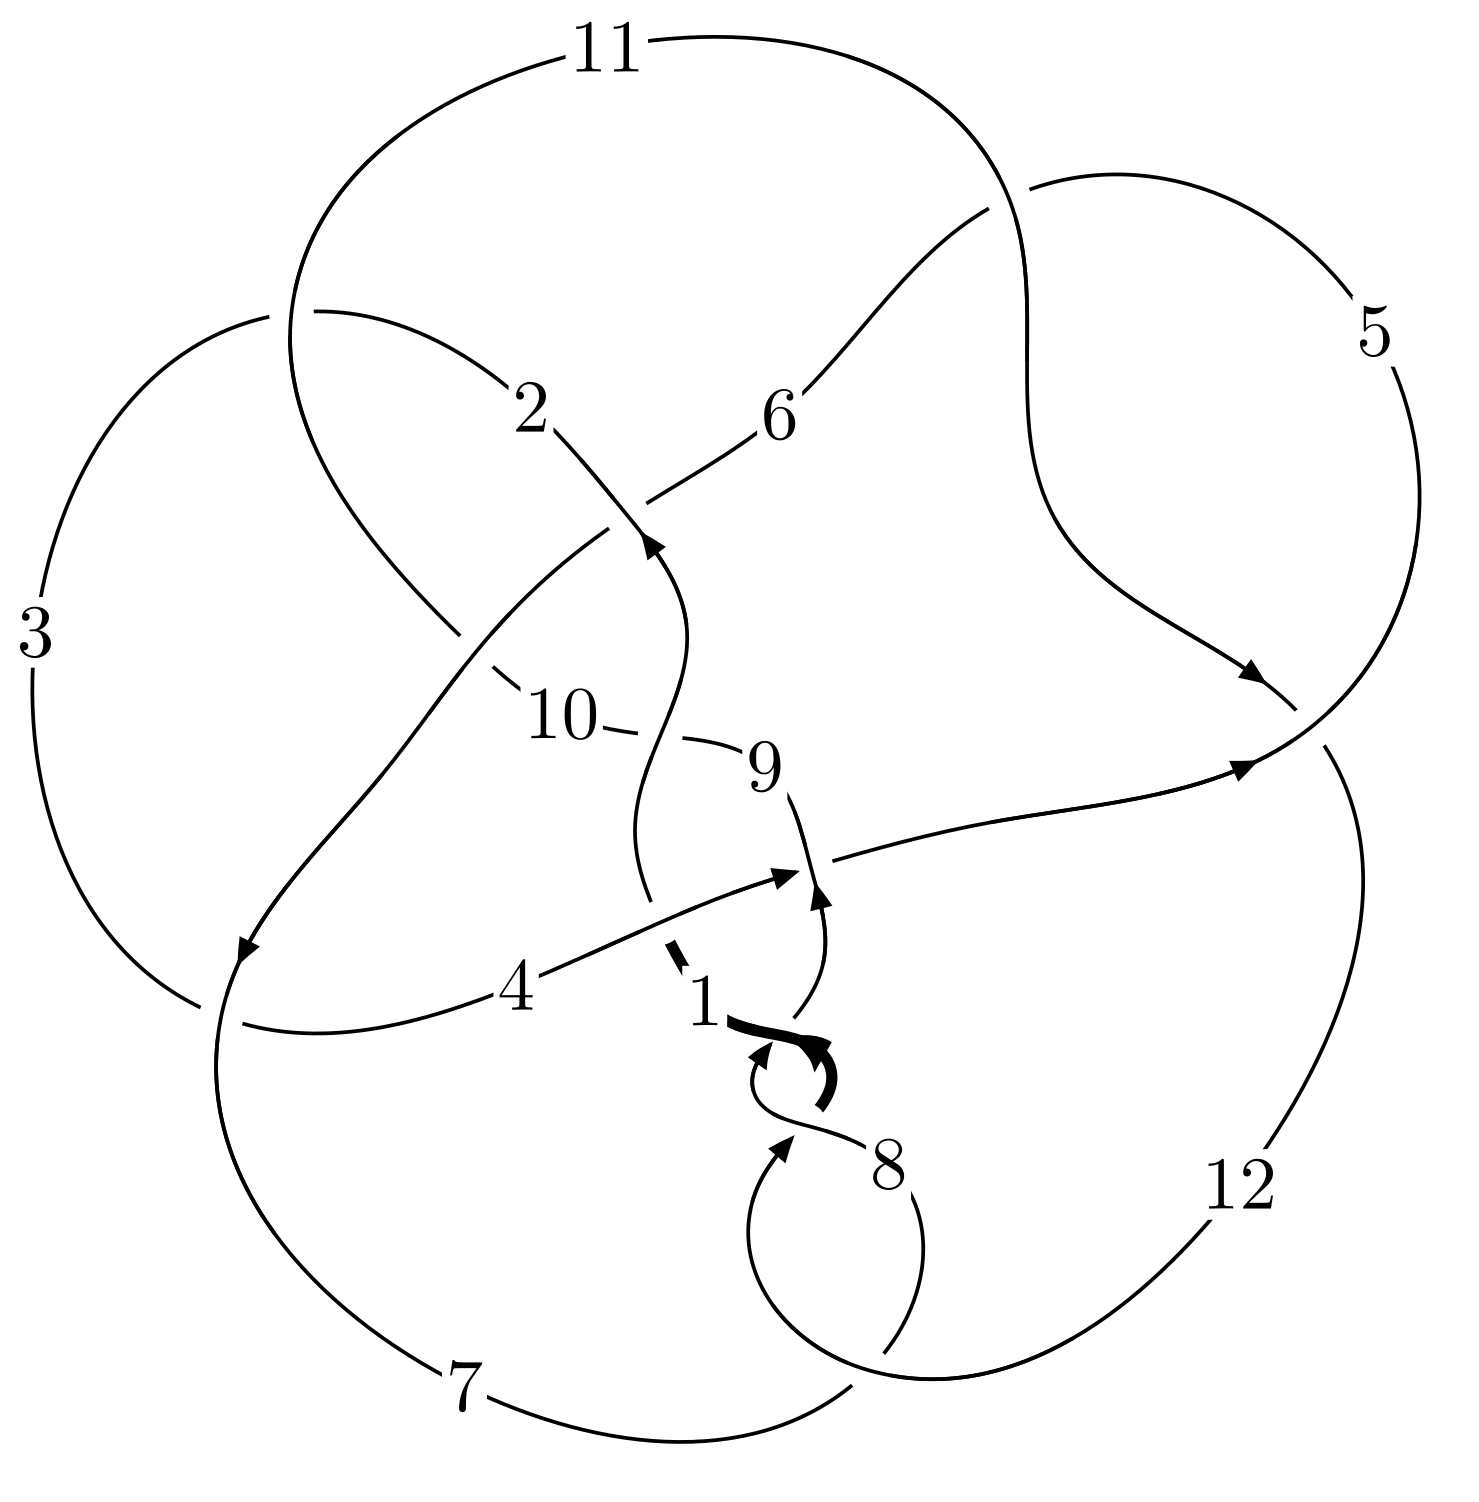
\includegraphics[width=112pt]{../../../GIT/diagram.site/Diagrams/png/2802_12n_0713.png}\\
\ \ \ A knot diagram\footnotemark}&
\allowdisplaybreaks
\textbf{Linearized knot diagam} \\
\cline{2-2}
 &
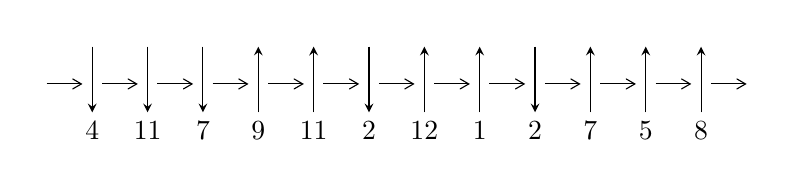
\begin{tikzpicture}[x=20pt, y=17pt]
	% nodes
	\node (C0) at (0, 0) {};
	\node (C1) at (1, 0) {};
	\node (C1U) at (1, +1) {};
	\node (C1D) at (1, -1) {4};

	\node (C2) at (2, 0) {};
	\node (C2U) at (2, +1) {};
	\node (C2D) at (2, -1) {11};

	\node (C3) at (3, 0) {};
	\node (C3U) at (3, +1) {};
	\node (C3D) at (3, -1) {7};

	\node (C4) at (4, 0) {};
	\node (C4U) at (4, +1) {};
	\node (C4D) at (4, -1) {9};

	\node (C5) at (5, 0) {};
	\node (C5U) at (5, +1) {};
	\node (C5D) at (5, -1) {11};

	\node (C6) at (6, 0) {};
	\node (C6U) at (6, +1) {};
	\node (C6D) at (6, -1) {2};

	\node (C7) at (7, 0) {};
	\node (C7U) at (7, +1) {};
	\node (C7D) at (7, -1) {12};

	\node (C8) at (8, 0) {};
	\node (C8U) at (8, +1) {};
	\node (C8D) at (8, -1) {1};

	\node (C9) at (9, 0) {};
	\node (C9U) at (9, +1) {};
	\node (C9D) at (9, -1) {2};

	\node (C10) at (10, 0) {};
	\node (C10U) at (10, +1) {};
	\node (C10D) at (10, -1) {7};

	\node (C11) at (11, 0) {};
	\node (C11U) at (11, +1) {};
	\node (C11D) at (11, -1) {5};

	\node (C12) at (12, 0) {};
	\node (C12U) at (12, +1) {};
	\node (C12D) at (12, -1) {8};
	\node (C13) at (13, 0) {};

	% arrows
	\draw[->,>={angle 60}]
	(C0) edge (C1) (C1) edge (C2) (C2) edge (C3) (C3) edge (C4) (C4) edge (C5) (C5) edge (C6) (C6) edge (C7) (C7) edge (C8) (C8) edge (C9) (C9) edge (C10) (C10) edge (C11) (C11) edge (C12) (C12) edge (C13) ;	\draw[->,>=stealth]
	(C1U) edge (C1D) (C2U) edge (C2D) (C3U) edge (C3D) (C4D) edge (C4U) (C5D) edge (C5U) (C6U) edge (C6D) (C7D) edge (C7U) (C8D) edge (C8U) (C9U) edge (C9D) (C10D) edge (C10U) (C11D) edge (C11U) (C12D) edge (C12U) ;
	\end{tikzpicture} \\
\hhline{~~} \\& 
\textbf{Solving Sequence} \\ \cline{2-2} 
 &
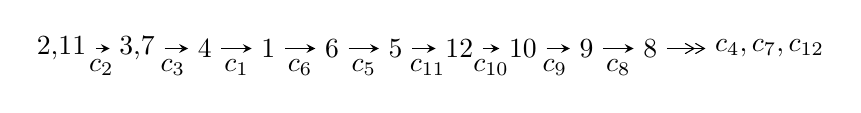
\begin{tikzpicture}[x=23pt, y=7pt]
	% node
	\node (A0) at (-1/8, 0) {2,11};
	\node (A1) at (17/16, 0) {3,7};
	\node (A2) at (17/8, 0) {4};
	\node (A3) at (25/8, 0) {1};
	\node (A4) at (33/8, 0) {6};
	\node (A5) at (41/8, 0) {5};
	\node (A6) at (49/8, 0) {12};
	\node (A7) at (57/8, 0) {10};
	\node (A8) at (65/8, 0) {9};
	\node (A9) at (73/8, 0) {8};
	\node (C1) at (1/2, -1) {$c_{2}$};
	\node (C2) at (13/8, -1) {$c_{3}$};
	\node (C3) at (21/8, -1) {$c_{1}$};
	\node (C4) at (29/8, -1) {$c_{6}$};
	\node (C5) at (37/8, -1) {$c_{5}$};
	\node (C6) at (45/8, -1) {$c_{11}$};
	\node (C7) at (53/8, -1) {$c_{10}$};
	\node (C8) at (61/8, -1) {$c_{9}$};
	\node (C9) at (69/8, -1) {$c_{8}$};
	\node (A10) at (11, 0) {$c_{4},c_{7},c_{12}$};

	% edge
	\draw[->,>=stealth]	
	(A0) edge (A1) (A1) edge (A2) (A2) edge (A3) (A3) edge (A4) (A4) edge (A5) (A5) edge (A6) (A6) edge (A7) (A7) edge (A8) (A8) edge (A9) ;
	\draw[->>,>={angle 60}]	
	(A9) edge (A10);
\end{tikzpicture} \\ 

\end{tabular} \\

\footnotetext{
The image of knot diagram is generated by the software ``\textbf{Draw programme}" developed by Andrew Bartholomew(\url{http://www.layer8.co.uk/maths/draw/index.htm\#Running-draw}), where we modified some parts for our purpose(\url{https://github.com/CATsTAILs/LinksPainter}).
}\phantom \\ \newline 
\centering \textbf{Ideals for irreducible components\footnotemark of $X_{\text{par}}$} 
 
\begin{align*}
I^u_{1}&=\langle 
2.57826\times10^{217} u^{63}-3.05321\times10^{217} u^{62}+\cdots+2.05878\times10^{220} b-1.16715\times10^{221},\\
\phantom{I^u_{1}}&\phantom{= \langle  }1.17201\times10^{218} u^{63}+2.06381\times10^{219} u^{62}+\cdots+8.44100\times10^{221} a+2.64039\times10^{222},\\
\phantom{I^u_{1}}&\phantom{= \langle  }u^{64}+38 u^{62}+\cdots-3396 u+328\rangle \\
I^u_{2}&=\langle 
-363987470832210 u^{18}+225606528026540 u^{17}+\cdots+4316043181765921 b-66280635064865,\\
\phantom{I^u_{2}}&\phantom{= \langle  }7.51222\times10^{15} u^{18}-5.60654\times10^{15} u^{17}+\cdots+3.88444\times10^{16} a+1.80154\times10^{16},\;u^{19}- u^{18}+\cdots+5 u-9\rangle \\
\\
\end{align*}
\raggedright * 2 irreducible components of $\dim_{\mathbb{C}}=0$, with total 83 representations.\\
\footnotetext{All coefficients of polynomials are rational numbers. But the coefficients are sometimes approximated in decimal forms when there is not enough margin.}
\newpage
\renewcommand{\arraystretch}{1}
\centering \section*{I. $I^u_{1}= \langle 2.58\times10^{217} u^{63}-3.05\times10^{217} u^{62}+\cdots+2.06\times10^{220} b-1.17\times10^{221},\;1.17\times10^{218} u^{63}+2.06\times10^{219} u^{62}+\cdots+8.44\times10^{221} a+2.64\times10^{222},\;u^{64}+38 u^{62}+\cdots-3396 u+328 \rangle$}
\flushleft \textbf{(i) Arc colorings}\\
\begin{tabular}{m{7pt} m{180pt} m{7pt} m{180pt} }
\flushright $a_{2}=$&$\begin{pmatrix}1\\0\end{pmatrix}$ \\
\flushright $a_{11}=$&$\begin{pmatrix}0\\u\end{pmatrix}$ \\
\flushright $a_{3}=$&$\begin{pmatrix}1\\u^2\end{pmatrix}$ \\
\flushright $a_{7}=$&$\begin{pmatrix}-0.000138847 u^{63}-0.00244499 u^{62}+\cdots+21.3318 u-3.12805\\-0.00125233 u^{63}+0.00148302 u^{62}+\cdots-41.5747 u+5.66913\end{pmatrix}$ \\
\flushright $a_{4}=$&$\begin{pmatrix}-0.00791855 u^{63}+0.00212409 u^{62}+\cdots-118.662 u+14.1417\\-0.00457474 u^{63}-0.000971202 u^{62}+\cdots-26.4167 u+2.01978\end{pmatrix}$ \\
\flushright $a_{1}=$&$\begin{pmatrix}-0.0135367 u^{63}-0.00367954 u^{62}+\cdots-88.7259 u+10.0079\\-0.00159543 u^{63}-0.00175310 u^{62}+\cdots+22.4981 u-3.38442\end{pmatrix}$ \\
\flushright $a_{6}=$&$\begin{pmatrix}-0.00139117 u^{63}-0.000961969 u^{62}+\cdots-20.2429 u+2.54108\\-0.00125233 u^{63}+0.00148302 u^{62}+\cdots-41.5747 u+5.66913\end{pmatrix}$ \\
\flushright $a_{5}=$&$\begin{pmatrix}-0.00139117 u^{63}-0.000961969 u^{62}+\cdots-20.2429 u+2.54108\\-0.00238057 u^{63}+0.000801163 u^{62}+\cdots-44.3852 u+5.98465\end{pmatrix}$ \\
\flushright $a_{12}=$&$\begin{pmatrix}0.0251528 u^{63}+0.00622070 u^{62}+\cdots+174.801 u-20.8026\\0.000927416 u^{63}+0.000804470 u^{62}+\cdots-5.52337 u+0.525490\end{pmatrix}$ \\
\flushright $a_{10}=$&$\begin{pmatrix}-0.0230195 u^{63}-0.00337024 u^{62}+\cdots-204.054 u+24.8603\\-0.00135242 u^{63}-0.00130024 u^{62}+\cdots+10.8548 u-1.49184\end{pmatrix}$ \\
\flushright $a_{9}=$&$\begin{pmatrix}-0.0243719 u^{63}-0.00467049 u^{62}+\cdots-193.200 u+23.3684\\-0.00135242 u^{63}-0.00130024 u^{62}+\cdots+10.8548 u-1.49184\end{pmatrix}$ \\
\flushright $a_{8}=$&$\begin{pmatrix}-0.0159602 u^{63}-0.00446479 u^{62}+\cdots-111.349 u+13.1348\\-0.000210627 u^{63}+0.000910006 u^{62}+\cdots-23.7656 u+3.66319\end{pmatrix}$\\&\end{tabular}
\flushleft \textbf{(ii) Obstruction class $= -1$}\\~\\
\flushleft \textbf{(iii) Cusp Shapes $= 0.0161918 u^{63}-0.00558987 u^{62}+\cdots+220.422 u-20.8374$}\\~\\
\newpage\renewcommand{\arraystretch}{1}
\flushleft \textbf{(iv) u-Polynomials at the component}\newline \\
\begin{tabular}{m{50pt}|m{274pt}}
Crossings & \hspace{64pt}u-Polynomials at each crossing \\
\hline $$\begin{aligned}c_{1}\end{aligned}$$&$\begin{aligned}
&u^{64}-7 u^{63}+\cdots-2062 u+473
\end{aligned}$\\
\hline $$\begin{aligned}c_{2}\end{aligned}$$&$\begin{aligned}
&u^{64}+38 u^{62}+\cdots+3396 u+328
\end{aligned}$\\
\hline $$\begin{aligned}c_{3}\end{aligned}$$&$\begin{aligned}
&u^{64}-3 u^{63}+\cdots-1741810 u-196291
\end{aligned}$\\
\hline $$\begin{aligned}c_{4}\end{aligned}$$&$\begin{aligned}
&u^{64}+3 u^{63}+\cdots-160 u-64
\end{aligned}$\\
\hline $$\begin{aligned}c_{5},c_{11}\end{aligned}$$&$\begin{aligned}
&u^{64}+13 u^{62}+\cdots-400 u+44
\end{aligned}$\\
\hline $$\begin{aligned}c_{6}\end{aligned}$$&$\begin{aligned}
&u^{64}+u^{63}+\cdots+6587 u+761
\end{aligned}$\\
\hline $$\begin{aligned}c_{7},c_{8},c_{12}\end{aligned}$$&$\begin{aligned}
&u^{64}+2 u^{63}+\cdots-14 u-1
\end{aligned}$\\
\hline $$\begin{aligned}c_{9}\end{aligned}$$&$\begin{aligned}
&u^{64}- u^{63}+\cdots-132 u-4
\end{aligned}$\\
\hline $$\begin{aligned}c_{10}\end{aligned}$$&$\begin{aligned}
&u^{64}+u^{63}+\cdots-1769 u+1279
\end{aligned}$\\
\hline
\end{tabular}\\~\\
\newpage\renewcommand{\arraystretch}{1}
\flushleft \textbf{(v) Riley Polynomials at the component}\newline \\
\begin{tabular}{m{50pt}|m{274pt}}
Crossings & \hspace{64pt}Riley Polynomials at each crossing \\
\hline $$\begin{aligned}c_{1}\end{aligned}$$&$\begin{aligned}
&y^{64}+25 y^{63}+\cdots+9011076 y+223729
\end{aligned}$\\
\hline $$\begin{aligned}c_{2}\end{aligned}$$&$\begin{aligned}
&y^{64}+76 y^{63}+\cdots+188592 y+107584
\end{aligned}$\\
\hline $$\begin{aligned}c_{3}\end{aligned}$$&$\begin{aligned}
&y^{64}+51 y^{63}+\cdots-510208710782 y+38530156681
\end{aligned}$\\
\hline $$\begin{aligned}c_{4}\end{aligned}$$&$\begin{aligned}
&y^{64}-11 y^{63}+\cdots-87040 y+4096
\end{aligned}$\\
\hline $$\begin{aligned}c_{5},c_{11}\end{aligned}$$&$\begin{aligned}
&y^{64}+26 y^{63}+\cdots+49616 y+1936
\end{aligned}$\\
\hline $$\begin{aligned}c_{6}\end{aligned}$$&$\begin{aligned}
&y^{64}+69 y^{63}+\cdots+3038519 y+579121
\end{aligned}$\\
\hline $$\begin{aligned}c_{7},c_{8},c_{12}\end{aligned}$$&$\begin{aligned}
&y^{64}-66 y^{63}+\cdots-16 y+1
\end{aligned}$\\
\hline $$\begin{aligned}c_{9}\end{aligned}$$&$\begin{aligned}
&y^{64}+17 y^{63}+\cdots-3936 y+16
\end{aligned}$\\
\hline $$\begin{aligned}c_{10}\end{aligned}$$&$\begin{aligned}
&y^{64}-87 y^{63}+\cdots-27241069 y+1635841
\end{aligned}$\\
\hline
\end{tabular}\\~\\
\newpage\flushleft \textbf{(vi) Complex Volumes and Cusp Shapes}
$$\begin{array}{c|c|c}  
\text{Solutions to }I^u_{1}& \I (\text{vol} + \sqrt{-1}CS) & \text{Cusp shape}\\
 \hline 
\begin{aligned}
u &= -0.335462 + 0.960170 I \\
a &= \phantom{-}0.595539 + 0.682559 I \\
b &= -0.963148 - 0.475228 I\end{aligned}
 & \phantom{-}0.911770 - 1.032120 I & \phantom{-}10.14320 + 0. I\phantom{ +0.000000I} \\ \hline\begin{aligned}
u &= -0.335462 - 0.960170 I \\
a &= \phantom{-}0.595539 - 0.682559 I \\
b &= -0.963148 + 0.475228 I\end{aligned}
 & \phantom{-}0.911770 + 1.032120 I & \phantom{-}10.14320 + 0. I\phantom{ +0.000000I} \\ \hline\begin{aligned}
u &= \phantom{-}0.947399 + 0.407862 I \\
a &= \phantom{-}0.338537 + 0.167075 I \\
b &= \phantom{-}0.248342 + 0.496214 I\end{aligned}
 & -1.74827 - 1.26516 I & \phantom{-0.000000 } 0 \\ \hline\begin{aligned}
u &= \phantom{-}0.947399 - 0.407862 I \\
a &= \phantom{-}0.338537 - 0.167075 I \\
b &= \phantom{-}0.248342 - 0.496214 I\end{aligned}
 & -1.74827 + 1.26516 I & \phantom{-0.000000 } 0 \\ \hline\begin{aligned}
u &= -0.083732 + 0.833478 I \\
a &= \phantom{-}1.045740 - 0.072964 I \\
b &= \phantom{-}0.415317 - 0.555202 I\end{aligned}
 & \phantom{-}3.87313 + 2.36028 I & \phantom{-}5.21332 - 3.90932 I \\ \hline\begin{aligned}
u &= -0.083732 - 0.833478 I \\
a &= \phantom{-}1.045740 + 0.072964 I \\
b &= \phantom{-}0.415317 + 0.555202 I\end{aligned}
 & \phantom{-}3.87313 - 2.36028 I & \phantom{-}5.21332 + 3.90932 I \\ \hline\begin{aligned}
u &= -0.274944 + 0.772279 I \\
a &= \phantom{-}0.790148 + 0.696555 I \\
b &= \phantom{-}0.900831 - 0.923664 I\end{aligned}
 & \phantom{-}3.41888 + 3.02488 I & \phantom{-}6.95291 - 3.41925 I \\ \hline\begin{aligned}
u &= -0.274944 - 0.772279 I \\
a &= \phantom{-}0.790148 - 0.696555 I \\
b &= \phantom{-}0.900831 + 0.923664 I\end{aligned}
 & \phantom{-}3.41888 - 3.02488 I & \phantom{-}6.95291 + 3.41925 I \\ \hline\begin{aligned}
u &= \phantom{-}0.075179 + 0.799821 I \\
a &= \phantom{-}0.467257 - 0.575187 I \\
b &= -1.259260 - 0.113697 I\end{aligned}
 & -0.99222 - 4.14641 I & \phantom{-}3.23080 + 6.97746 I \\ \hline\begin{aligned}
u &= \phantom{-}0.075179 - 0.799821 I \\
a &= \phantom{-}0.467257 + 0.575187 I \\
b &= -1.259260 + 0.113697 I\end{aligned}
 & -0.99222 + 4.14641 I & \phantom{-}3.23080 - 6.97746 I\\
 \hline 
 \end{array}$$\newpage$$\begin{array}{c|c|c}  
\text{Solutions to }I^u_{1}& \I (\text{vol} + \sqrt{-1}CS) & \text{Cusp shape}\\
 \hline 
\begin{aligned}
u &= \phantom{-}0.413467 + 1.150880 I \\
a &= \phantom{-}0.144937 - 1.402750 I \\
b &= -0.04335 + 1.55505 I\end{aligned}
 & \phantom{-}8.44712 - 3.02698 I & \phantom{-0.000000 } 0 \\ \hline\begin{aligned}
u &= \phantom{-}0.413467 - 1.150880 I \\
a &= \phantom{-}0.144937 + 1.402750 I \\
b &= -0.04335 - 1.55505 I\end{aligned}
 & \phantom{-}8.44712 + 3.02698 I & \phantom{-0.000000 } 0 \\ \hline\begin{aligned}
u &= \phantom{-}0.040362 + 0.770178 I \\
a &= \phantom{-}0.243807 + 0.579784 I \\
b &= -1.365740 + 0.360315 I\end{aligned}
 & \phantom{-}4.98892 + 8.36284 I & \phantom{-}6.61798 - 6.58755 I \\ \hline\begin{aligned}
u &= \phantom{-}0.040362 - 0.770178 I \\
a &= \phantom{-}0.243807 - 0.579784 I \\
b &= -1.365740 - 0.360315 I\end{aligned}
 & \phantom{-}4.98892 - 8.36284 I & \phantom{-}6.61798 + 6.58755 I \\ \hline\begin{aligned}
u &= \phantom{-}0.642406 + 0.395793 I \\
a &= \phantom{-}0.539832 + 0.618893 I \\
b &= \phantom{-}0.406004 + 0.585662 I\end{aligned}
 & -1.72328 - 1.35345 I & \phantom{-}2.84079 + 5.01791 I \\ \hline\begin{aligned}
u &= \phantom{-}0.642406 - 0.395793 I \\
a &= \phantom{-}0.539832 - 0.618893 I \\
b &= \phantom{-}0.406004 - 0.585662 I\end{aligned}
 & -1.72328 + 1.35345 I & \phantom{-}2.84079 - 5.01791 I \\ \hline\begin{aligned}
u &= -1.24948\phantom{ +0.000000I} \\
a &= \phantom{-}0.543935\phantom{ +0.000000I} \\
b &= \phantom{-}0.299788\phantom{ +0.000000I}\end{aligned}
 & \phantom{-}2.44452\phantom{ +0.000000I} & \phantom{-0.000000 } 0 \\ \hline\begin{aligned}
u &= -0.647244 + 0.349890 I \\
a &= -1.55678 + 1.74713 I \\
b &= \phantom{-}0.254178 - 0.482779 I\end{aligned}
 & \phantom{-}3.51271 - 6.62719 I & \phantom{-}6.97914 + 1.82931 I \\ \hline\begin{aligned}
u &= -0.647244 - 0.349890 I \\
a &= -1.55678 - 1.74713 I \\
b &= \phantom{-}0.254178 + 0.482779 I\end{aligned}
 & \phantom{-}3.51271 + 6.62719 I & \phantom{-}6.97914 - 1.82931 I \\ \hline\begin{aligned}
u &= -1.313910 + 0.215826 I \\
a &= -0.220902 + 0.147842 I \\
b &= \phantom{-}0.039760 - 0.791805 I\end{aligned}
 & -1.70737 + 4.39848 I & \phantom{-0.000000 } 0\\
 \hline 
 \end{array}$$\newpage$$\begin{array}{c|c|c}  
\text{Solutions to }I^u_{1}& \I (\text{vol} + \sqrt{-1}CS) & \text{Cusp shape}\\
 \hline 
\begin{aligned}
u &= -1.313910 - 0.215826 I \\
a &= -0.220902 - 0.147842 I \\
b &= \phantom{-}0.039760 + 0.791805 I\end{aligned}
 & -1.70737 - 4.39848 I & \phantom{-0.000000 } 0 \\ \hline\begin{aligned}
u &= -1.002620 + 0.901051 I \\
a &= \phantom{-}0.650289 - 0.114573 I \\
b &= \phantom{-}0.489302 - 0.434084 I\end{aligned}
 & \phantom{-}2.48875 + 1.68278 I & \phantom{-0.000000 } 0 \\ \hline\begin{aligned}
u &= -1.002620 - 0.901051 I \\
a &= \phantom{-}0.650289 + 0.114573 I \\
b &= \phantom{-}0.489302 + 0.434084 I\end{aligned}
 & \phantom{-}2.48875 - 1.68278 I & \phantom{-0.000000 } 0 \\ \hline\begin{aligned}
u &= \phantom{-}0.21372 + 1.41112 I \\
a &= -0.482160 + 1.217250 I \\
b &= \phantom{-}0.00954 - 1.79768 I\end{aligned}
 & \phantom{-}6.23466 - 0.00352 I & \phantom{-0.000000 } 0 \\ \hline\begin{aligned}
u &= \phantom{-}0.21372 - 1.41112 I \\
a &= -0.482160 - 1.217250 I \\
b &= \phantom{-}0.00954 + 1.79768 I\end{aligned}
 & \phantom{-}6.23466 + 0.00352 I & \phantom{-0.000000 } 0 \\ \hline\begin{aligned}
u &= -0.329023 + 0.401985 I \\
a &= \phantom{-}0.975551 + 0.406906 I \\
b &= -0.291314 + 0.190827 I\end{aligned}
 & \phantom{-}1.055720 - 0.384090 I & \phantom{-}8.69250 + 1.65178 I \\ \hline\begin{aligned}
u &= -0.329023 - 0.401985 I \\
a &= \phantom{-}0.975551 - 0.406906 I \\
b &= -0.291314 - 0.190827 I\end{aligned}
 & \phantom{-}1.055720 + 0.384090 I & \phantom{-}8.69250 - 1.65178 I \\ \hline\begin{aligned}
u &= -0.513200\phantom{ +0.000000I} \\
a &= \phantom{-}0.799271\phantom{ +0.000000I} \\
b &= \phantom{-}1.40728\phantom{ +0.000000I}\end{aligned}
 & \phantom{-}1.44268\phantom{ +0.000000I} & \phantom{-}14.7350\phantom{ +0.000000I} \\ \hline\begin{aligned}
u &= -0.45260 + 1.42133 I \\
a &= -0.683739 - 1.056290 I \\
b &= \phantom{-}0.08781 + 1.76465 I\end{aligned}
 & \phantom{-}11.76650 + 4.51689 I & \phantom{-0.000000 } 0 \\ \hline\begin{aligned}
u &= -0.45260 - 1.42133 I \\
a &= -0.683739 + 1.056290 I \\
b &= \phantom{-}0.08781 - 1.76465 I\end{aligned}
 & \phantom{-}11.76650 - 4.51689 I & \phantom{-0.000000 } 0\\
 \hline 
 \end{array}$$\newpage$$\begin{array}{c|c|c}  
\text{Solutions to }I^u_{1}& \I (\text{vol} + \sqrt{-1}CS) & \text{Cusp shape}\\
 \hline 
\begin{aligned}
u &= \phantom{-}0.204121 + 0.364148 I \\
a &= \phantom{-}1.076330 - 0.192389 I \\
b &= \phantom{-}0.905084 + 0.351582 I\end{aligned}
 & -1.66720 - 0.88112 I & -0.76201 - 1.29100 I \\ \hline\begin{aligned}
u &= \phantom{-}0.204121 - 0.364148 I \\
a &= \phantom{-}1.076330 + 0.192389 I \\
b &= \phantom{-}0.905084 - 0.351582 I\end{aligned}
 & -1.66720 + 0.88112 I & -0.76201 + 1.29100 I \\ \hline\begin{aligned}
u &= \phantom{-}1.58492 + 0.27627 I \\
a &= -0.296423 - 0.332935 I \\
b &= -0.051364 + 0.836910 I\end{aligned}
 & \phantom{-}4.76022 - 7.21958 I & \phantom{-0.000000 } 0 \\ \hline\begin{aligned}
u &= \phantom{-}1.58492 - 0.27627 I \\
a &= -0.296423 + 0.332935 I \\
b &= -0.051364 - 0.836910 I\end{aligned}
 & \phantom{-}4.76022 + 7.21958 I & \phantom{-0.000000 } 0 \\ \hline\begin{aligned}
u &= \phantom{-}0.291913 + 0.225982 I \\
a &= -3.00732 - 2.80629 I \\
b &= \phantom{-}0.436516 + 0.467769 I\end{aligned}
 & -2.93293 + 3.01950 I & \phantom{-}3.23967 - 1.03009 I \\ \hline\begin{aligned}
u &= \phantom{-}0.291913 - 0.225982 I \\
a &= -3.00732 + 2.80629 I \\
b &= \phantom{-}0.436516 - 0.467769 I\end{aligned}
 & -2.93293 - 3.01950 I & \phantom{-}3.23967 + 1.03009 I \\ \hline\begin{aligned}
u &= \phantom{-}0.192418 + 0.305935 I \\
a &= \phantom{-}1.86300 - 1.16501 I \\
b &= -0.457918 - 0.710588 I\end{aligned}
 & \phantom{-}7.58427 + 2.24555 I & \phantom{-}8.62267 - 0.85529 I \\ \hline\begin{aligned}
u &= \phantom{-}0.192418 - 0.305935 I \\
a &= \phantom{-}1.86300 + 1.16501 I \\
b &= -0.457918 + 0.710588 I\end{aligned}
 & \phantom{-}7.58427 - 2.24555 I & \phantom{-}8.62267 + 0.85529 I \\ \hline\begin{aligned}
u &= \phantom{-}0.01286 + 1.66235 I \\
a &= -0.251779 - 1.041480 I \\
b &= \phantom{-}0.03327 + 1.75492 I\end{aligned}
 & \phantom{-}7.78730 - 4.22834 I & \phantom{-0.000000 } 0 \\ \hline\begin{aligned}
u &= \phantom{-}0.01286 - 1.66235 I \\
a &= -0.251779 + 1.041480 I \\
b &= \phantom{-}0.03327 - 1.75492 I\end{aligned}
 & \phantom{-}7.78730 + 4.22834 I & \phantom{-0.000000 } 0\\
 \hline 
 \end{array}$$\newpage$$\begin{array}{c|c|c}  
\text{Solutions to }I^u_{1}& \I (\text{vol} + \sqrt{-1}CS) & \text{Cusp shape}\\
 \hline 
\begin{aligned}
u &= \phantom{-}0.39994 + 1.64387 I \\
a &= \phantom{-}0.177619 - 0.870097 I \\
b &= \phantom{-}0.38697 + 1.58361 I\end{aligned}
 & \phantom{-}2.98425 - 4.18476 I & \phantom{-0.000000 } 0 \\ \hline\begin{aligned}
u &= \phantom{-}0.39994 - 1.64387 I \\
a &= \phantom{-}0.177619 + 0.870097 I \\
b &= \phantom{-}0.38697 - 1.58361 I\end{aligned}
 & \phantom{-}2.98425 + 4.18476 I & \phantom{-0.000000 } 0 \\ \hline\begin{aligned}
u &= \phantom{-}0.283207 + 0.080826 I \\
a &= -1.44066 - 3.30718 I \\
b &= \phantom{-}0.589344 - 0.669131 I\end{aligned}
 & -1.97533 + 1.42210 I & \phantom{-}0.91620 - 6.10321 I \\ \hline\begin{aligned}
u &= \phantom{-}0.283207 - 0.080826 I \\
a &= -1.44066 + 3.30718 I \\
b &= \phantom{-}0.589344 + 0.669131 I\end{aligned}
 & -1.97533 - 1.42210 I & \phantom{-}0.91620 + 6.10321 I \\ \hline\begin{aligned}
u &= \phantom{-}0.24314 + 1.68834 I \\
a &= \phantom{-}0.056309 + 1.169580 I \\
b &= -0.58798 - 1.65311 I\end{aligned}
 & \phantom{-}5.49499 - 5.40830 I & \phantom{-0.000000 } 0 \\ \hline\begin{aligned}
u &= \phantom{-}0.24314 - 1.68834 I \\
a &= \phantom{-}0.056309 - 1.169580 I \\
b &= -0.58798 + 1.65311 I\end{aligned}
 & \phantom{-}5.49499 + 5.40830 I & \phantom{-0.000000 } 0 \\ \hline\begin{aligned}
u &= -0.16084 + 1.73860 I \\
a &= \phantom{-}0.230933 + 0.972132 I \\
b &= \phantom{-}0.307850 - 1.361670 I\end{aligned}
 & \phantom{-}4.47021 + 1.14177 I & \phantom{-0.000000 } 0 \\ \hline\begin{aligned}
u &= -0.16084 - 1.73860 I \\
a &= \phantom{-}0.230933 - 0.972132 I \\
b &= \phantom{-}0.307850 + 1.361670 I\end{aligned}
 & \phantom{-}4.47021 - 1.14177 I & \phantom{-0.000000 } 0 \\ \hline\begin{aligned}
u &= -0.67469 + 1.61833 I \\
a &= \phantom{-}0.214372 + 1.071080 I \\
b &= \phantom{-}0.09629 - 1.53447 I\end{aligned}
 & \phantom{-}5.14768 + 3.33362 I & \phantom{-0.000000 } 0 \\ \hline\begin{aligned}
u &= -0.67469 - 1.61833 I \\
a &= \phantom{-}0.214372 - 1.071080 I \\
b &= \phantom{-}0.09629 + 1.53447 I\end{aligned}
 & \phantom{-}5.14768 - 3.33362 I & \phantom{-0.000000 } 0\\
 \hline 
 \end{array}$$\newpage$$\begin{array}{c|c|c}  
\text{Solutions to }I^u_{1}& \I (\text{vol} + \sqrt{-1}CS) & \text{Cusp shape}\\
 \hline 
\begin{aligned}
u &= -0.49546 + 1.71265 I \\
a &= \phantom{-}0.092150 + 0.806725 I \\
b &= \phantom{-}0.36691 - 1.75692 I\end{aligned}
 & \phantom{-}8.17146 + 6.66450 I & \phantom{-0.000000 } 0 \\ \hline\begin{aligned}
u &= -0.49546 - 1.71265 I \\
a &= \phantom{-}0.092150 - 0.806725 I \\
b &= \phantom{-}0.36691 + 1.75692 I\end{aligned}
 & \phantom{-}8.17146 - 6.66450 I & \phantom{-0.000000 } 0 \\ \hline\begin{aligned}
u &= -0.43824 + 1.74966 I \\
a &= -0.035433 - 1.125870 I \\
b &= -0.53312 + 1.71047 I\end{aligned}
 & \phantom{-}5.15081 + 11.10080 I & \phantom{-0.000000 } 0 \\ \hline\begin{aligned}
u &= -0.43824 - 1.74966 I \\
a &= -0.035433 + 1.125870 I \\
b &= -0.53312 - 1.71047 I\end{aligned}
 & \phantom{-}5.15081 - 11.10080 I & \phantom{-0.000000 } 0 \\ \hline\begin{aligned}
u &= \phantom{-}0.07921 + 1.82792 I \\
a &= \phantom{-}0.167616 - 1.054340 I \\
b &= -0.53046 + 1.46401 I\end{aligned}
 & \phantom{-}13.45120 + 1.32917 I & \phantom{-0.000000 } 0 \\ \hline\begin{aligned}
u &= \phantom{-}0.07921 - 1.82792 I \\
a &= \phantom{-}0.167616 + 1.054340 I \\
b &= -0.53046 - 1.46401 I\end{aligned}
 & \phantom{-}13.45120 - 1.32917 I & \phantom{-0.000000 } 0 \\ \hline\begin{aligned}
u &= \phantom{-}0.05911 + 1.89435 I \\
a &= -0.290232 + 0.899724 I \\
b &= \phantom{-}0.02290 - 1.79203 I\end{aligned}
 & \phantom{-}14.7249 + 6.6669 I & \phantom{-0.000000 } 0 \\ \hline\begin{aligned}
u &= \phantom{-}0.05911 - 1.89435 I \\
a &= -0.290232 - 0.899724 I \\
b &= \phantom{-}0.02290 + 1.79203 I\end{aligned}
 & \phantom{-}14.7249 - 6.6669 I & \phantom{-0.000000 } 0 \\ \hline\begin{aligned}
u &= \phantom{-}0.54843 + 1.85229 I \\
a &= -0.061480 + 1.071260 I \\
b &= -0.49609 - 1.73014 I\end{aligned}
 & \phantom{-}11.8878 - 15.3498 I & \phantom{-0.000000 } 0 \\ \hline\begin{aligned}
u &= \phantom{-}0.54843 - 1.85229 I \\
a &= -0.061480 - 1.071260 I \\
b &= -0.49609 + 1.73014 I\end{aligned}
 & \phantom{-}11.8878 + 15.3498 I & \phantom{-0.000000 } 0\\
 \hline 
 \end{array}$$\newpage$$\begin{array}{c|c|c}  
\text{Solutions to }I^u_{1}& \I (\text{vol} + \sqrt{-1}CS) & \text{Cusp shape}\\
 \hline 
\begin{aligned}
u &= \phantom{-}0.91204 + 1.79319 I \\
a &= \phantom{-}0.271605 - 1.004440 I \\
b &= \phantom{-}0.10036 + 1.51621 I\end{aligned}
 & \phantom{-}10.63020 - 4.22345 I & \phantom{-0.000000 } 0 \\ \hline\begin{aligned}
u &= \phantom{-}0.91204 - 1.79319 I \\
a &= \phantom{-}0.271605 + 1.004440 I \\
b &= \phantom{-}0.10036 - 1.51621 I\end{aligned}
 & \phantom{-}10.63020 + 4.22345 I & \phantom{-0.000000 } 0 \\ \hline\begin{aligned}
u &= -0.05374 + 2.23789 I \\
a &= \phantom{-}0.164957 - 1.018210 I \\
b &= \phantom{-}0.129617 + 1.231340 I\end{aligned}
 & \phantom{-}12.37100 - 0.19756 I & \phantom{-0.000000 } 0 \\ \hline\begin{aligned}
u &= -0.05374 - 2.23789 I \\
a &= \phantom{-}0.164957 + 1.018210 I \\
b &= \phantom{-}0.129617 - 1.231340 I\end{aligned}
 & \phantom{-}12.37100 + 0.19756 I & \phantom{-0.000000 } 0\\
 \hline 
 \end{array}$$\newpage\newpage\renewcommand{\arraystretch}{1}
\centering \section*{II. $I^u_{2}= \langle -3.64\times10^{14} u^{18}+2.26\times10^{14} u^{17}+\cdots+4.32\times10^{15} b-6.63\times10^{13},\;7.51\times10^{15} u^{18}-5.61\times10^{15} u^{17}+\cdots+3.88\times10^{16} a+1.80\times10^{16},\;u^{19}- u^{18}+\cdots+5 u-9 \rangle$}
\flushleft \textbf{(i) Arc colorings}\\
\begin{tabular}{m{7pt} m{180pt} m{7pt} m{180pt} }
\flushright $a_{2}=$&$\begin{pmatrix}1\\0\end{pmatrix}$ \\
\flushright $a_{11}=$&$\begin{pmatrix}0\\u\end{pmatrix}$ \\
\flushright $a_{3}=$&$\begin{pmatrix}1\\u^2\end{pmatrix}$ \\
\flushright $a_{7}=$&$\begin{pmatrix}-0.193393 u^{18}+0.144333 u^{17}+\cdots-2.35275 u-0.463784\\0.0843336 u^{18}-0.0522716 u^{17}+\cdots+0.789469 u+0.0153568\end{pmatrix}$ \\
\flushright $a_{4}=$&$\begin{pmatrix}0.109059 u^{18}-0.0920616 u^{17}+\cdots+1.56328 u+2.44843\\-0.0485297 u^{18}+0.110929 u^{17}+\cdots-0.896544 u+0.847023\end{pmatrix}$ \\
\flushright $a_{1}=$&$\begin{pmatrix}0.192472 u^{18}-0.326504 u^{17}+\cdots+2.51451 u-1.68558\\-0.0459865 u^{18}-0.101011 u^{17}+\cdots+0.541386 u-1.38026\end{pmatrix}$ \\
\flushright $a_{6}=$&$\begin{pmatrix}-0.109059 u^{18}+0.0920616 u^{17}+\cdots-1.56328 u-0.448427\\0.0843336 u^{18}-0.0522716 u^{17}+\cdots+0.789469 u+0.0153568\end{pmatrix}$ \\
\flushright $a_{5}=$&$\begin{pmatrix}-0.109059 u^{18}+0.0920616 u^{17}+\cdots-1.56328 u-0.448427\\0.0358039 u^{18}+0.0586574 u^{17}+\cdots-0.107076 u-0.137620\end{pmatrix}$ \\
\flushright $a_{12}=$&$\begin{pmatrix}0.00205396 u^{18}+0.179383 u^{17}+\cdots-2.72735 u+1.54621\\0.187705 u^{18}+0.0524445 u^{17}+\cdots+0.697793 u+2.93670\end{pmatrix}$ \\
\flushright $a_{10}=$&$\begin{pmatrix}0.151338 u^{18}-0.164905 u^{17}+\cdots+2.78710 u+0.861192\\-0.0419331 u^{18}-0.0288332 u^{17}+\cdots+1.52675 u-1.10364\end{pmatrix}$ \\
\flushright $a_{9}=$&$\begin{pmatrix}0.109405 u^{18}-0.193738 u^{17}+\cdots+4.31384 u-0.242445\\-0.0419331 u^{18}-0.0288332 u^{17}+\cdots+1.52675 u-1.10364\end{pmatrix}$ \\
\flushright $a_{8}=$&$\begin{pmatrix}-0.112709 u^{18}+0.299193 u^{17}+\cdots-0.988091 u+2.55979\\0.0604367 u^{18}+0.175102 u^{17}+\cdots+0.648882 u+2.74600\end{pmatrix}$\\&\end{tabular}
\flushleft \textbf{(ii) Obstruction class $= 1$}\\~\\
\flushleft \textbf{(iii) Cusp Shapes $= -\frac{4159791503582966}{4316043181765921} u^{18}+\frac{2428875393014454}{4316043181765921} u^{17}+\cdots-\frac{60944556846167549}{4316043181765921} u-\frac{39429270153907668}{4316043181765921}$}\\~\\
\newpage\renewcommand{\arraystretch}{1}
\flushleft \textbf{(iv) u-Polynomials at the component}\newline \\
\begin{tabular}{m{50pt}|m{274pt}}
Crossings & \hspace{64pt}u-Polynomials at each crossing \\
\hline $$\begin{aligned}c_{1}\end{aligned}$$&$\begin{aligned}
&u^{19}-6 u^{18}+\cdots+3 u-1
\end{aligned}$\\
\hline $$\begin{aligned}c_{2}\end{aligned}$$&$\begin{aligned}
&u^{19}- u^{18}+\cdots+5 u-9
\end{aligned}$\\
\hline $$\begin{aligned}c_{3}\end{aligned}$$&$\begin{aligned}
&u^{19}+2 u^{18}+\cdots+15 u-9
\end{aligned}$\\
\hline $$\begin{aligned}c_{4}\end{aligned}$$&$\begin{aligned}
&u^{19}+u^{17}+\cdots+u+1
\end{aligned}$\\
\hline $$\begin{aligned}c_{5}\end{aligned}$$&$\begin{aligned}
&u^{19}- u^{18}+\cdots-22 u^2-4
\end{aligned}$\\
\hline $$\begin{aligned}c_{6}\end{aligned}$$&$\begin{aligned}
&u^{19}+4 u^{18}+\cdots-2 u+1
\end{aligned}$\\
\hline $$\begin{aligned}c_{7},c_{8}\end{aligned}$$&$\begin{aligned}
&u^{19}+u^{18}+\cdots+3 u+1
\end{aligned}$\\
\hline $$\begin{aligned}c_{9}\end{aligned}$$&$\begin{aligned}
&u^{19}- u^{17}+\cdots+4 u+4
\end{aligned}$\\
\hline $$\begin{aligned}c_{10}\end{aligned}$$&$\begin{aligned}
&u^{19}+2 u^{18}+\cdots+4 u+1
\end{aligned}$\\
\hline $$\begin{aligned}c_{11}\end{aligned}$$&$\begin{aligned}
&u^{19}+u^{18}+\cdots+22 u^2+4
\end{aligned}$\\
\hline $$\begin{aligned}c_{12}\end{aligned}$$&$\begin{aligned}
&u^{19}- u^{18}+\cdots+3 u-1
\end{aligned}$\\
\hline
\end{tabular}\\~\\
\newpage\renewcommand{\arraystretch}{1}
\flushleft \textbf{(v) Riley Polynomials at the component}\newline \\
\begin{tabular}{m{50pt}|m{274pt}}
Crossings & \hspace{64pt}Riley Polynomials at each crossing \\
\hline $$\begin{aligned}c_{1}\end{aligned}$$&$\begin{aligned}
&y^{19}+6 y^{18}+\cdots-7 y-1
\end{aligned}$\\
\hline $$\begin{aligned}c_{2}\end{aligned}$$&$\begin{aligned}
&y^{19}+13 y^{18}+\cdots+439 y-81
\end{aligned}$\\
\hline $$\begin{aligned}c_{3}\end{aligned}$$&$\begin{aligned}
&y^{19}+20 y^{18}+\cdots-405 y-81
\end{aligned}$\\
\hline $$\begin{aligned}c_{4}\end{aligned}$$&$\begin{aligned}
&y^{19}+2 y^{18}+\cdots+y-1
\end{aligned}$\\
\hline $$\begin{aligned}c_{5},c_{11}\end{aligned}$$&$\begin{aligned}
&y^{19}+15 y^{18}+\cdots-176 y-16
\end{aligned}$\\
\hline $$\begin{aligned}c_{6}\end{aligned}$$&$\begin{aligned}
&y^{19}+10 y^{18}+\cdots+10 y-1
\end{aligned}$\\
\hline $$\begin{aligned}c_{7},c_{8},c_{12}\end{aligned}$$&$\begin{aligned}
&y^{19}-21 y^{18}+\cdots-11 y-1
\end{aligned}$\\
\hline $$\begin{aligned}c_{9}\end{aligned}$$&$\begin{aligned}
&y^{19}-2 y^{18}+\cdots+96 y-16
\end{aligned}$\\
\hline $$\begin{aligned}c_{10}\end{aligned}$$&$\begin{aligned}
&y^{19}-14 y^{18}+\cdots+30 y-1
\end{aligned}$\\
\hline
\end{tabular}\\~\\
\newpage\flushleft \textbf{(vi) Complex Volumes and Cusp Shapes}
$$\begin{array}{c|c|c}  
\text{Solutions to }I^u_{2}& \I (\text{vol} + \sqrt{-1}CS) & \text{Cusp shape}\\
 \hline 
\begin{aligned}
u &= \phantom{-}0.389083 + 0.971159 I \\
a &= -0.277741 + 0.595285 I \\
b &= \phantom{-}0.932245 - 0.473799 I\end{aligned}
 & \phantom{-}0.46032 + 1.43826 I & -0.20028 - 4.42405 I \\ \hline\begin{aligned}
u &= \phantom{-}0.389083 - 0.971159 I \\
a &= -0.277741 - 0.595285 I \\
b &= \phantom{-}0.932245 + 0.473799 I\end{aligned}
 & \phantom{-}0.46032 - 1.43826 I & -0.20028 + 4.42405 I \\ \hline\begin{aligned}
u &= -0.800104 + 0.507328 I \\
a &= \phantom{-}0.388644 - 0.220349 I \\
b &= \phantom{-}0.710720 - 0.420295 I\end{aligned}
 & -2.27973 + 1.36896 I & -12.95881 - 5.08171 I \\ \hline\begin{aligned}
u &= -0.800104 - 0.507328 I \\
a &= \phantom{-}0.388644 + 0.220349 I \\
b &= \phantom{-}0.710720 + 0.420295 I\end{aligned}
 & -2.27973 - 1.36896 I & -12.95881 + 5.08171 I \\ \hline\begin{aligned}
u &= -0.914926 + 0.042064 I \\
a &= \phantom{-}0.09423 + 1.49670 I \\
b &= -0.539979 - 0.327295 I\end{aligned}
 & \phantom{-}2.77115 - 7.45545 I & \phantom{-}1.04337 + 6.84145 I \\ \hline\begin{aligned}
u &= -0.914926 - 0.042064 I \\
a &= \phantom{-}0.09423 - 1.49670 I \\
b &= -0.539979 + 0.327295 I\end{aligned}
 & \phantom{-}2.77115 + 7.45545 I & \phantom{-}1.04337 - 6.84145 I \\ \hline\begin{aligned}
u &= \phantom{-}0.947057 + 0.591059 I \\
a &= \phantom{-}0.473404 + 0.014503 I \\
b &= \phantom{-}0.810839 + 0.917232 I\end{aligned}
 & \phantom{-}2.33987 - 2.91659 I & -0.25529 + 5.05539 I \\ \hline\begin{aligned}
u &= \phantom{-}0.947057 - 0.591059 I \\
a &= \phantom{-}0.473404 - 0.014503 I \\
b &= \phantom{-}0.810839 - 0.917232 I\end{aligned}
 & \phantom{-}2.33987 + 2.91659 I & -0.25529 - 5.05539 I \\ \hline\begin{aligned}
u &= \phantom{-}0.818159\phantom{ +0.000000I} \\
a &= \phantom{-}0.221354\phantom{ +0.000000I} \\
b &= \phantom{-}1.21245\phantom{ +0.000000I}\end{aligned}
 & \phantom{-}1.07163\phantom{ +0.000000I} & -8.02200\phantom{ +0.000000I} \\ \hline\begin{aligned}
u &= -0.555367 + 0.570698 I \\
a &= \phantom{-}1.55276 - 0.46301 I \\
b &= -0.470414 - 0.688016 I\end{aligned}
 & -1.79164 - 0.64199 I & \phantom{-}4.02276 - 3.01754 I\\
 \hline 
 \end{array}$$\newpage$$\begin{array}{c|c|c}  
\text{Solutions to }I^u_{2}& \I (\text{vol} + \sqrt{-1}CS) & \text{Cusp shape}\\
 \hline 
\begin{aligned}
u &= -0.555367 - 0.570698 I \\
a &= \phantom{-}1.55276 + 0.46301 I \\
b &= -0.470414 + 0.688016 I\end{aligned}
 & -1.79164 + 0.64199 I & \phantom{-}4.02276 + 3.01754 I \\ \hline\begin{aligned}
u &= \phantom{-}0.699603 + 0.245787 I \\
a &= \phantom{-}0.80766 + 1.51414 I \\
b &= -0.486775 + 0.028785 I\end{aligned}
 & -3.49065 - 3.76561 I & -3.11008 + 7.06177 I \\ \hline\begin{aligned}
u &= \phantom{-}0.699603 - 0.245787 I \\
a &= \phantom{-}0.80766 - 1.51414 I \\
b &= -0.486775 - 0.028785 I\end{aligned}
 & -3.49065 + 3.76561 I & -3.11008 - 7.06177 I \\ \hline\begin{aligned}
u &= \phantom{-}0.70448 + 1.41196 I \\
a &= \phantom{-}0.305323 - 0.963046 I \\
b &= \phantom{-}0.00641 + 1.66974 I\end{aligned}
 & \phantom{-}9.00068 - 4.71241 I & \phantom{-}5.89823 + 4.68766 I \\ \hline\begin{aligned}
u &= \phantom{-}0.70448 - 1.41196 I \\
a &= \phantom{-}0.305323 + 0.963046 I \\
b &= \phantom{-}0.00641 - 1.66974 I\end{aligned}
 & \phantom{-}9.00068 + 4.71241 I & \phantom{-}5.89823 - 4.68766 I \\ \hline\begin{aligned}
u &= -0.47470 + 1.61232 I \\
a &= \phantom{-}0.160463 + 1.124330 I \\
b &= \phantom{-}0.17424 - 1.56147 I\end{aligned}
 & \phantom{-}5.05062 + 2.83722 I & \phantom{-}3.41245 + 2.37831 I \\ \hline\begin{aligned}
u &= -0.47470 - 1.61232 I \\
a &= \phantom{-}0.160463 - 1.124330 I \\
b &= \phantom{-}0.17424 + 1.56147 I\end{aligned}
 & \phantom{-}5.05062 - 2.83722 I & \phantom{-}3.41245 - 2.37831 I \\ \hline\begin{aligned}
u &= \phantom{-}0.09579 + 2.08758 I \\
a &= -0.004309 - 1.065310 I \\
b &= \phantom{-}0.256494 + 1.250070 I\end{aligned}
 & \phantom{-}12.07760 - 1.14448 I & \phantom{-}4.65867 + 5.51636 I \\ \hline\begin{aligned}
u &= \phantom{-}0.09579 - 2.08758 I \\
a &= -0.004309 + 1.065310 I \\
b &= \phantom{-}0.256494 - 1.250070 I\end{aligned}
 & \phantom{-}12.07760 + 1.14448 I & \phantom{-}4.65867 - 5.51636 I\\
 \hline 
 \end{array}$$\newpage
\newpage\renewcommand{\arraystretch}{1}
\centering \section*{ III. u-Polynomials}
\begin{tabular}{m{50pt}|m{274pt}}
Crossings & \hspace{64pt}u-Polynomials at each crossing \\
\hline $$\begin{aligned}c_{1}\end{aligned}$$&$\begin{aligned}
&(u^{19}-6 u^{18}+\cdots+3 u-1)(u^{64}-7 u^{63}+\cdots-2062 u+473)
\end{aligned}$\\
\hline $$\begin{aligned}c_{2}\end{aligned}$$&$\begin{aligned}
&(u^{19}- u^{18}+\cdots+5 u-9)(u^{64}+38 u^{62}+\cdots+3396 u+328)
\end{aligned}$\\
\hline $$\begin{aligned}c_{3}\end{aligned}$$&$\begin{aligned}
&(u^{19}+2 u^{18}+\cdots+15 u-9)(u^{64}-3 u^{63}+\cdots-1741810 u-196291)
\end{aligned}$\\
\hline $$\begin{aligned}c_{4}\end{aligned}$$&$\begin{aligned}
&(u^{19}+u^{17}+\cdots+u+1)(u^{64}+3 u^{63}+\cdots-160 u-64)
\end{aligned}$\\
\hline $$\begin{aligned}c_{5}\end{aligned}$$&$\begin{aligned}
&(u^{19}- u^{18}+\cdots-22 u^2-4)(u^{64}+13 u^{62}+\cdots-400 u+44)
\end{aligned}$\\
\hline $$\begin{aligned}c_{6}\end{aligned}$$&$\begin{aligned}
&(u^{19}+4 u^{18}+\cdots-2 u+1)(u^{64}+u^{63}+\cdots+6587 u+761)
\end{aligned}$\\
\hline $$\begin{aligned}c_{7},c_{8}\end{aligned}$$&$\begin{aligned}
&(u^{19}+u^{18}+\cdots+3 u+1)(u^{64}+2 u^{63}+\cdots-14 u-1)
\end{aligned}$\\
\hline $$\begin{aligned}c_{9}\end{aligned}$$&$\begin{aligned}
&(u^{19}- u^{17}+\cdots+4 u+4)(u^{64}- u^{63}+\cdots-132 u-4)
\end{aligned}$\\
\hline $$\begin{aligned}c_{10}\end{aligned}$$&$\begin{aligned}
&(u^{19}+2 u^{18}+\cdots+4 u+1)(u^{64}+u^{63}+\cdots-1769 u+1279)
\end{aligned}$\\
\hline $$\begin{aligned}c_{11}\end{aligned}$$&$\begin{aligned}
&(u^{19}+u^{18}+\cdots+22 u^2+4)(u^{64}+13 u^{62}+\cdots-400 u+44)
\end{aligned}$\\
\hline $$\begin{aligned}c_{12}\end{aligned}$$&$\begin{aligned}
&(u^{19}- u^{18}+\cdots+3 u-1)(u^{64}+2 u^{63}+\cdots-14 u-1)
\end{aligned}$\\
\hline
\end{tabular}\newpage\renewcommand{\arraystretch}{1}
\centering \section*{ IV. Riley Polynomials}
\begin{tabular}{m{50pt}|m{274pt}}
Crossings & \hspace{64pt}Riley Polynomials at each crossing \\
\hline $$\begin{aligned}c_{1}\end{aligned}$$&$\begin{aligned}
&(y^{19}+6 y^{18}+\cdots-7 y-1)(y^{64}+25 y^{63}+\cdots+9011076 y+223729)
\end{aligned}$\\
\hline $$\begin{aligned}c_{2}\end{aligned}$$&$\begin{aligned}
&(y^{19}+13 y^{18}+\cdots+439 y-81)\\
&\cdot(y^{64}+76 y^{63}+\cdots+188592 y+107584)
\end{aligned}$\\
\hline $$\begin{aligned}c_{3}\end{aligned}$$&$\begin{aligned}
&(y^{19}+20 y^{18}+\cdots-405 y-81)\\
&\cdot(y^{64}+51 y^{63}+\cdots-510208710782 y+38530156681)
\end{aligned}$\\
\hline $$\begin{aligned}c_{4}\end{aligned}$$&$\begin{aligned}
&(y^{19}+2 y^{18}+\cdots+y-1)(y^{64}-11 y^{63}+\cdots-87040 y+4096)
\end{aligned}$\\
\hline $$\begin{aligned}c_{5},c_{11}\end{aligned}$$&$\begin{aligned}
&(y^{19}+15 y^{18}+\cdots-176 y-16)(y^{64}+26 y^{63}+\cdots+49616 y+1936)
\end{aligned}$\\
\hline $$\begin{aligned}c_{6}\end{aligned}$$&$\begin{aligned}
&(y^{19}+10 y^{18}+\cdots+10 y-1)\\
&\cdot(y^{64}+69 y^{63}+\cdots+3038519 y+579121)
\end{aligned}$\\
\hline $$\begin{aligned}c_{7},c_{8},c_{12}\end{aligned}$$&$\begin{aligned}
&(y^{19}-21 y^{18}+\cdots-11 y-1)(y^{64}-66 y^{63}+\cdots-16 y+1)
\end{aligned}$\\
\hline $$\begin{aligned}c_{9}\end{aligned}$$&$\begin{aligned}
&(y^{19}-2 y^{18}+\cdots+96 y-16)(y^{64}+17 y^{63}+\cdots-3936 y+16)
\end{aligned}$\\
\hline $$\begin{aligned}c_{10}\end{aligned}$$&$\begin{aligned}
&(y^{19}-14 y^{18}+\cdots+30 y-1)\\
&\cdot(y^{64}-87 y^{63}+\cdots-27241069 y+1635841)
\end{aligned}$\\
\hline
\end{tabular}
\vskip 2pc
\end{document}